\section{Arduino}
\subsection{Ausstattung}
Um den Zielen, die wir uns für unseren Prototypen gesetzt haben, gerecht zu werden, ist der Arduino mit einem Sim 808 Module sowie entsprechenden GPS und GSM Antennen ausgerüstet.
\\
\\
Verbunden sind das Modul und die Antennen mit Hilfe eines Shields. Es handelt sich um ein Shield des Models OAS808SIM und ist von der Firma MakerFabs.
\\
\\
Die Stromversorgung erfolgt mittels vier BRC 18650 4200mAh Batterien, die in Reihe geschaltet sind. 
\subsection{Software}
Die Kontrolle des Shields erfolgt mittels UART und entsprechenden AT-Befehlen. Die erforderlichen Befehle sind zusammen mit einer kurzen Erklärung nachfolgend  in den Abbildungen \ref{Gsm_http} und \ref{GPS} aufgelistet.

\begin{figure} [H]
 \begin{center}
		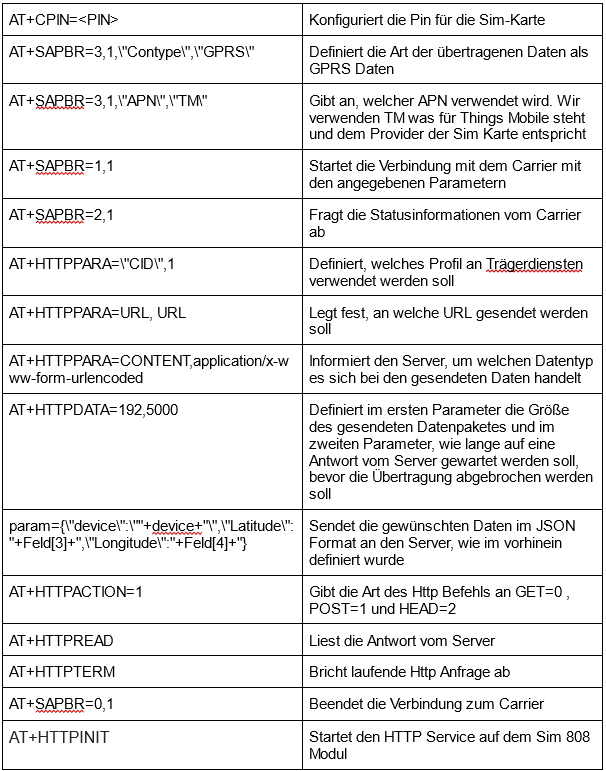
\includegraphics[width=1\textwidth]{Bilder/Arduino_Befehlstabelle_1.png}
		\caption{GSM und Http-Befehle}
		\label{Gsm_http}
	\end{center}
\end{figure}
\begin{figure} [H]
 \begin{center}
		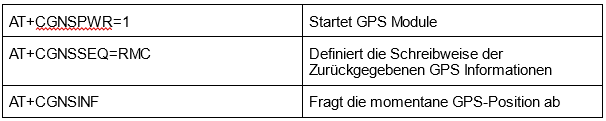
\includegraphics[width=1\textwidth]{Bilder/Arduino_Befehlstabelle_2.png}
		\caption{GPS-Befehle}
		\label{GPS}
	\end{center}
\end{figure}
\subsection{Aufbau Code}
Der Code ist wie ein Standard-Mikrocontroller-Code aufgebaut und besitzt zwei Unterfunktionen, die hier kurz grafisch in Abbildung \ref{PAP} dargestellt werden.
\begin{figure} [H]
	\begin{center}
		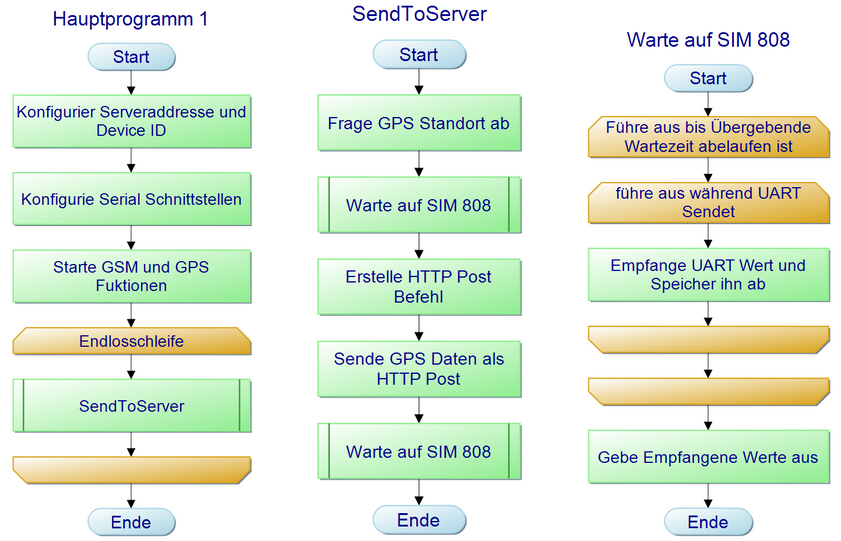
\includegraphics[width=1\textwidth]{Bilder/Arduino_Codeaufbau.png}
		\caption{Programmablaufplan}
		\label{PAP}
	\end{center}
\end{figure}
Der Arduino macht in der momentanen Prototyp Version nichts anderes, als das Sim 808 Modul zu steuern. Dafür gibt es drei Funktionen:
\\
\\
Eine Funktion, welche die Kommunikation mit dem Sim Modul erleichtert, eine weitere Funktion für die Abfrage des momentanen Standortes und eine dritte, um die Kommunikation mit dem Server zu erlauben. 
\\
\\
Mit der Funktion wart() wird zum einen das Pausieren für die Bearbeitungszeiträume geliefert und zum anderen die Ausgabe des Sim Moduls an den PC zum Debuggen geschickt. 
Die Funktion gpsDaten fragt den aktuellen Standort ab und die Funktion SendToServer sendet die zu übermittelnden GPS Daten an den Server.
Der Code ist in C geschrieben, da diese Programmiersprache für unsere Zwecke ausreichend performant ist.

\subsection{Entwicklungsprozess}
Der Entwicklungsprozess ist in mehreren Stufen erfolgt. Zunächst wurde mittels eines einfachen Programms die Funktionalität der GPS-Antenne überprüft, da wir dafür noch keine Sim-Karte benötigten. Zur Implementierung der Standortabfrage soll zum ersten Mal die UART-Schnittstelle zum Board konfiguriert werden. Nachdem die UART-Schnittstelle konfiguriert wurde, haben wir die Funktion wart() entwickelt, um die Kommunikation mit der UART-Schnittstelle zu erleichtern. Mit Hilfe der wart() Funktion konnten wir nun auf die Antwort von der UART-Schnittstelle warten und dies auf dem Computer zum Debuggen ausgeben. Das Senden und Empfangen von Informationen über UART funktionierte also und anschließend haben wir die Abfrage der GPS-Daten realisiert. Nachdem wir die entsprechenden Befehle gefunden hatten, war dies einfach zu realisieren.
\\
\\
Da die ersten Tests jedoch auf dem Dachboden ausgeführt wurden und das Dach aus Metall ist, konnte zunächst kein Signal empfangen werden. Nachdem wir das Problem erkannt hatten, haben wir alle zukünftigen Test an einer besser geeigneten Position durchgeführt.
\\
\\
Die Standortabfrage funktionierte nun, sodass wir im nächsten Schritt zum Testen des GSM-Moduls und der Sim-Karte das Senden von SMS realisiert hatten. An dieser Stelle haben wir lediglich die bereits erstellten Funktionen genutzt und die Befehle für die SMS-Kommunikation hinzugefügt. Dabei ist aufgefallen, dass beim erstmaligen Nutzen des GSM-Moduls nach dem Einschalten immer der PIN zum Entsperren erforderlich ist. 
\\
\\
Nachdem wir die Kommunikation mit dem GSM Modul ermöglicht hatten, haben wir die Kommunikation mit dem Server realisiert.
Nachdem wir hierfür die richtigen Befehle gefunden hatten, haben wir zunächst Testdaten per HTTP POST an einen Test-Server gesendet, der einfach nur seine empfangen HTTP POSTs anzeigt. Danach haben wir das Senden von Daten im JSON-Format an unseren Server realisiert. Aus Netzwerksicht mussten wir nur die Serveradresse ändern.  Damit der Server die empfangenden Daten nutzen kann, mussten wir dann jedoch noch den Daten-Sendebefehl neu konfigurieren. Da wir über die UART-Schnittstelle nur Strings schicken können, mussten wir die Formatierung für die zu sendenden Daten anders einstellen und diese  dann beim versendeten String berücksichtigen. 
\\
\\
Nachdem die Kommunikation mit dem Server erfolgreich funktioniert hatte, haben wir die einzelnen Teile zusammengefügt. Hierfür mussten wir den GPS-Antwort-String verarbeiten. Um die benötigten Werte zu erhalten, haben wir den String immer an den Kommata in kleinere Strings unterteilt und über die vordefinierte Struktur des Strings ermittelt, welche Werte der Längengrad und der Breitengrad sind. Dies Werte haben wir für zukünftige Erweiterungen beziehungsweise Funktionalitäten zwischengespeichert und binden diese in den zu sendenden String ein.
\\
\\
Wir haben dabei den Datentyp String der erhaltenen Daten bewusst nicht geändert, da dies sonst dazu führt, dass Nachkommastellen weggelassen werden, was die Standortbestimmung verzerrt.
\subsection{Aufbau Hardware}
Für die Stromversorgung müssen die Akkus an den Vin (\textit{Eingangsspannung}) Pin und den GND (\textit{Masse}) Pin angeschlossen werden. Da das Shield diese Pins einfach durch schaltet, können wir die Konstruktion trotz Shield so verwenden.
\begin{figure} [H]
	\begin{center}
		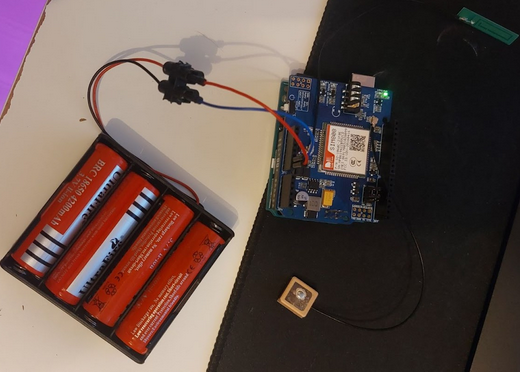
\includegraphics[width=1\textwidth]{Bilder/Arduino_Aufbau.png}
		\caption{Systemaufbau für das KFZ}
		\label{hw-system}
	\end{center}
\end{figure}
Der Vorteil dieser Konstruktion ist, dass sie sehr kompakt ist und somit leichter im Auto versteckt werden kann. Ein weiterer Vorteil dieser Bauweise ist, dass für den Fall, dass später durch Erweiterungen die Akkulaufzeit nicht ausreicht, einfach weitere Akkus parallel hinzugefügt werden können.

\subsection{Probleme}
Die Probleme, die bei der Entwicklung des Controllers aufgetreten sind, lassen sich in zwei Kategorien unterteilen. Zum einen gab es technische Probleme und zum anderen logistische Schwierigkeiten.
Das Problem bei der Beschaffung der GSM-Module war, dass diese meist aus China importiert werden mussten, was dazu geführt hat, dass wir unter langen Wartezeiten gelitten haben. Von den vier bestellten Modulen wurden zwei nicht geliefert (\textit{die Bestellung wurde vom Lieferanten gecancelt}). Des Weiteren konnte eines der Module nur über eine bereitgestellte Software verwendet werden.
\\
\\
Die technischen Probleme sind zum Teil auf die schlechte Dokumentation des Arduino Shields zurückzuführen. Zum einen fehlt die Information für die richtige Baudrate für die UART Schnittstelle, welche über strukturiertes Testen herausgefunden werden musste. Das Problem hierbei war, dass das Modul entsprechend keine Fehlermeldung zurückgeben konnte, da die Kommunikation zwischen Modul und Arduino selbst gestört war und  nichts zurückgeben wurde:
\begin{figure} [H]
	\begin{center}
		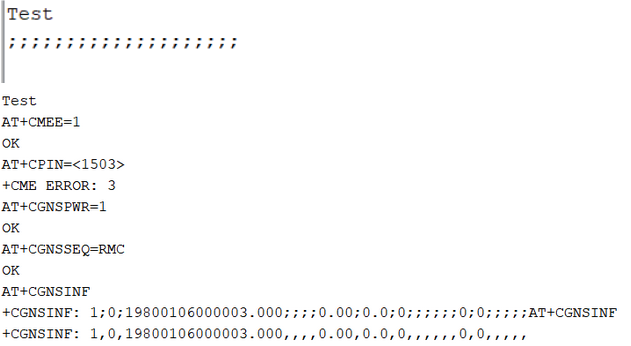
\includegraphics[width=1\textwidth]{Bilder/Arduino_Probleme.png}
		\caption{fehlerhafte und korrekte Ausgabe}
		\label{Arduinoproblem}
	\end{center}
\end{figure}
In Abbildung \ref{Arduinoproblem} sieht man zunächst, wie die fehlerhafte Ausgabe aussieht. Unter dieser ist zm Vergleich die richtige Ausgabe abgebildet.
\\
\\
Auch die AT-Befehle, welche zur Kommunikation mittels HTTP dienen sollten, haben nicht entsprechend funktioniert. Gelöst werden konnte das Problem, indem die Befehlskette verwendet wird, mit der jedes Datenpaket einzeln und manuell konfiguriert werden kann. Entsprechend mussten die Pakete als IOT-HTTP-Paket definiert werden und die Netzbetreiber-Daten sowie Paketinformationen für die Verbindung eingestellt werden.
\\
\\
Des weiteren hat das GSM-Modul die Kommunikation mit einer normalen Vodafone Sim-Karte nicht aufbauen können. Die Verzögerung, eine geeignete Prepaid Karte zu bekommen, hat den Zeitrahmen für diesen Teil erheblich nach hinten verschoben.
Das Problem an diesem Fehlern war, dass das Modul nur ERROR 3 zurückgegeben hat, was als \textit{“Operation nicht erlaubt”} definiert ist. Es wird dabei aber nicht genauer spezifiziert, warum diese Operation nicht erlaubt ist. Dies hat das Troubleshooting weiter erschwert.
\\
\\
Für die GPS-Abfrage haben sich zwei wesentliche Probleme ergeben. Das am schwierigsten zu lösende Problem war, dass die benötigten Befehle nicht in der richtigen Dokumentation zu finden sind, sondern nur in einigen Beispiel-Programmen vom Shield Hersteller. Das andere Problem ist, dass das GPS-Signal beim ersten Konfigurieren (\textit{Einstellen der internen Uhr}) guten Empfang braucht.

